\documentclass{report}
\usepackage[utf8]{inputenc}
\usepackage[english]{babel}
\usepackage{url}
\usepackage[left=1.1in,right=1.1in,top=1.5in,bottom=1.5in]{geometry}
\setlength{\parindent}{0pt}
\usepackage{tikz,stackengine}
\usepackage{lmodern}
\usepackage{tabularx}
\usepackage{amssymb}
\usepackage{amsmath}
\usepackage{enumitem}
\usepackage{algorithm}
\usepackage{algorithmic}
\usepackage{hyperref}
\renewcommand{\familydefault}{\sfdefault}
\usepackage{fancyhdr}
\pagestyle{fancy}
\fancyhf{}
\rhead{\large 190050023,190050030,190050051,190050106.}
\lhead{\large Design and Analysis of Algorithms}
\rfoot{\large Page \thepage}
\renewcommand{\headrulewidth}{1.5pt}
\renewcommand{\footrulewidth}{1.5pt}
\newcommand{\answerbox}[1]{\fbox{\rule{0.8in}{0pt}\textbf{#1}\rule[-0.25ex]{0pt}{3.5ex}}}
\usetikzlibrary{shapes,arrows}
\usetikzlibrary{arrows.meta}
\tikzstyle{sink} = [diamond, draw, fill=brown!20, 
    text width=2.5em, text badly centered, node distance=1.5cm, inner sep=0pt]
\tikzstyle{cloud} = [draw, ellipse,fill=blue!20, node distance=1cm,minimum height=1.2em]
\tikzstyle{lemma} = [rectangle,draw,fill=black!20, text badly centered,node distance=16cm,minimum height=2em,minimum width=16cm]
\begin{document}
 \rule[0mm]{16cm}{0.4pt}
 \begin{center}%
  {\LARGE Assignment - 3\par}%
 \end{center}%
 \par
 \begin{center}
 {\rule[0mm]{8cm}{0.4pt}}
 \end{center}
 \begin{center}%
  {\LARGE 17 April 2021 \par}%
 \end{center}
 \begin{center}
 {\rule[0mm]{8cm}{0.4pt}}
 \end{center}
 \begin{center}
  \large 190050023 \rule[0.5mm]{1cm}{0pt} Aquib Nawaz\par
 \end{center}
 \begin{center}
  \large 190050030 \rule[0.5mm]{0.9cm}{0pt} Rajesh Dasari\par
 \end{center}
 \begin{center}
  \large 190050051 \rule[0.5mm]{0.8cm}{0pt}Paavan Kumar\par
 \end{center}
 \begin{center}
  \large 190050106 \rule[0.5mm]{0.4cm}{0pt} Sanjana Burman\par
  \rule[0mm]{8cm}{0.4pt}
 \end{center}
 \rule[12mm]{16cm}{0.4pt}
 \section*{Question 1}
 \subsection*{a)}
 We Construct the Graph \textbf{G} by giving its  vertices \textbf{V}, edges \textbf{E}, and capacities \textbf{c} : \textbf{E} $\rightarrow$ $\mathbb{N}$\\
 \vspace*{1.2em}\\
 \rule[0.5cm]{2cm}{0pt} Let \textbf{P} be the set of all Persons and \textbf{J} be the set of all Jobs\\
 \rule[0.5mm]{2cm}{0pt} \textbf{V} = \{s\} $\cup$ \{t\} $\cup$ \{P$_i$ $|$ i $\in$ \textbf{P}\} $\cup$ \{J$_j$ $|$ j $\in$ \textbf{J}\} \\
 \vspace*{1.2em}\\
 \rule[0.5mm]{2cm}{0pt} Let \textbf{T} be all those pairs (i,j) where ith person is willing to do jth Job.\\
 \rule[0.5mm]{2cm}{0pt} \textbf{E} = \textbf{E$_{s}$} $\cup$ \textbf{E$_{m}$} $\cup$  \textbf{E$_{t}$} where\\
 \begin{equation*}
     \mathbf{E}_s = \{(s,P_i)\  |\  i \in \mathbf{P}\} 
 \end{equation*}
 \begin{equation*}
     \mathbf{E}_m = \{(P_i,J_j)\  | \ (i,j) \in \mathbf{T} \}
 \end{equation*}
 \begin{equation*}
     \mathbf{E}_t = \{(J_j,t)\ |\  j \in \mathbf{J}\}
 \end{equation*}
  \rule[0.5mm]{2cm}{0pt} The map \textbf{c} is defined as follows \\
   \[   
    \textbf{c(e)} = 
         \begin{cases}
           1 &\quad\text{if e} \in \mathbf{E}_s\\
           1 &\quad\text{if e} \in \mathbf{E}_m\\
           1 &\quad\text{if e} \in \mathbf{E}_t\\
         \end{cases}
    \]
 \newpage
 For example, one such graph would be as follows.\\
 \begin{center}
 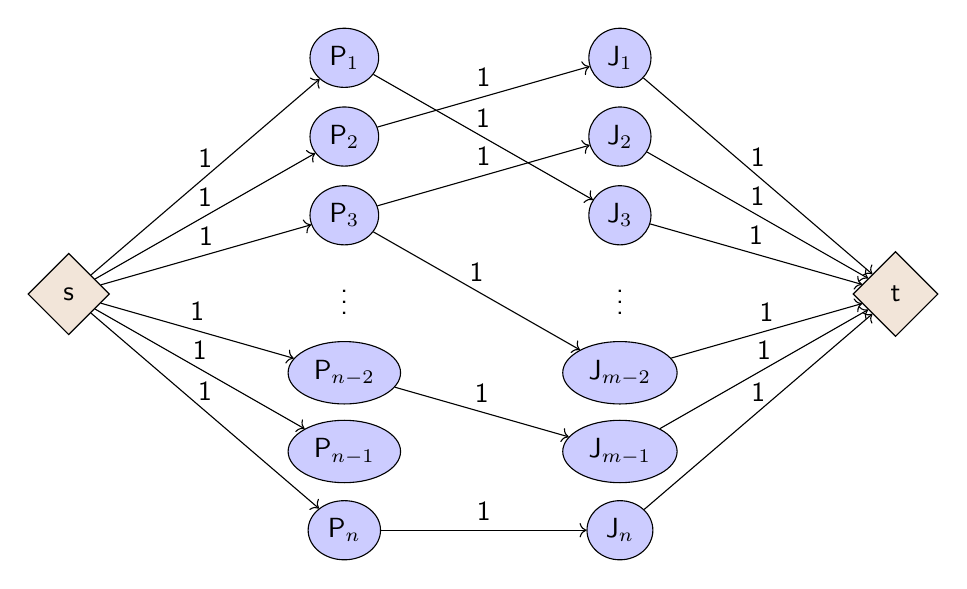
\begin{tikzpicture}[main/.style = {draw, circle}] 
    \node[sink] (1) {s};
    \node (2) [right of=1, node distance=3.5cm]  {$\vdots$};
    \node[cloud] (3) [above of=2,node distance=1cm] {P$_3$};
    \node[cloud] (9) [right of=3,node distance=3.5cm] {J$_3$};
    \node[cloud] (4) [above of=3,node distance=1cm] {P$_2$};
    \node[cloud] (10) [right of=4,node distance=3.5cm] {J$_2$};
    \node[cloud] (5) [below of=2,node distance=1cm] {P$_{n-2}$};
    \node[cloud] (11) [right of=5,node distance=3.5cm] {J$_{m-2}$};
    \node[cloud] (6) [below of=5,node distance=1cm] {P$_{n-1}$};
    \node[cloud] (12) [right of=6,node distance=3.5cm] {J$_{m-1}$};
    \node[cloud] (7) [below of=6,node distance=1cm] {P$_n$};
    \node[cloud] (13) [right of=7,node distance=3.5cm] {J$_n$};
    \node[cloud] (8) [above of=4,node distance=1cm] {P$_1$};
    \node[cloud] (14) [right of=8,node distance=3.5cm] {J$_1$};
    \node (15) [right of=2, node distance=3.5cm]  {$\vdots$};
    \node[sink] (16) [right of=15,node distance=3.5cm] {t};
    %\draw[->] (1) -- node[midway,above]{$\infty$} (2);
    \draw[->] (1) -- node[midway,above]{1} (3);
    \draw[->] (1) -- node[midway,above]{1} (4);
    \draw[->] (1) -- node[midway,above]{1} (5);
    \draw[->] (1) -- node[midway,above]{1} (6);
    \draw[->] (1) -- node[midway,above]{1} (7);
    \draw[->] (1) -- node[midway,above]{1} (8);
    \draw[<-] (16) -- node[midway,above]{1} (9);
    \draw[<-] (16) -- node[midway,above]{1} (10);
    \draw[<-] (16) -- node[midway,above]{1} (11);
    \draw[<-] (16) -- node[midway,above]{1} (12);
    \draw[<-] (16) -- node[midway,above]{1} (13);
    \draw[<-] (16) -- node[midway,above]{1} (14);
    \draw[->] (3) -- node[midway,above]{1} (11);
    \draw[->] (4) -- node[midway,above]{1} (14);
    \draw[->] (5) -- node[midway,above]{1} (12);
    \draw[->] (3) -- node[midway,above]{1} (10);
    \draw[->] (7) -- node[midway,above]{1} (13);
    \draw[->] (8) -- node[midway,above]{1} (9);
 \end{tikzpicture}
 \end{center}
 For Some \textbf{integer} valued flow in the Graph \textbf{G} we have the following a person is assigned a Job if \textbf{f}(P$_i$,J$_j$) = 1 
 \begin{enumerate}
     \item Such a Flow assignment has no person getting assigned more than 1 Job.
     \begin{itemize}
         \item This is due to Flow conservation at Person nodes
         \item Therefore at most one Job can be assigned since there is only incoming edge with capacity 1 which means a single outgoing edge with capacity 1.
     \end{itemize}
     \item Such a Flow assignment has a person getting assigned the Job he is willing to do.
     \begin{itemize}
         \item This is due to the construction of the graph.
         \item Edges are present in the main graph if and only if a person is willing to do the Job
     \end{itemize}
     \item Such a Flow Assignment has \textbf{f}(J$_j$,t) = 1 if and only if J$_j$ is assigned.
     \begin{itemize}
         \item This is due to Flow conservation at Job Nodes
         \item If a Job is assigned to a person P$_i$ that means there is an incoming edge with \textbf{f}(P$_i$,J$_j$) = 1
         \item Since only one outgoing edge its flow value \textbf{f}(J$_j$,t) must also be 1 and this job is not assigned to any other person except the person P$_i$
     \end{itemize}
 \end{enumerate}
 \boxed{\text{\large\textbf{Lemma} : \textbf{G} has a flow of value $n$ if and only if all the jobs are assigned}}  \\
    \vspace*{0em}\\
 \textbf{Proof} : Suppose \textbf{G} has a flow of size n. ($\implies$)\vspace{0.5em}\\
 \rule[0.5mm]{1.1cm}{0pt} This means that \textbf{f}(j,t) = 1 for j $\in$ \textbf{E}$_t$\\
 \rule[0.5cm]{1.1cm}{0pt} Hence All Jobs are assigned.\\
 \rule[0.5cm]{1.1cm}{0pt} Suppose all Jobs are not assigned.($\impliedby$)\\
 \rule[0.5cm]{1.1cm}{0pt} This means that there is some Job j that is not assigned\\
 \rule[0.5cm]{1.1cm}{0pt} Hence \textbf{f}(j,t) = 0  which means $|\mathbf{f}|$ = \textbf{f}$^\gets$(t) = $\sum_1^n$ \textbf{f}(j,t) $<$ n\\
 \subsection*{b)}
 We Construct the Graph \textbf{G} by giving its  vertices \textbf{V}, edges \textbf{E}, and capacities \textbf{c} : \textbf{E} $\rightarrow$ $\mathbb{N}$\\
 \vspace*{1.2em}\\
 \rule[0.5cm]{2cm}{0pt} Let \textbf{P} be the set of all Persons and \textbf{J} be the set of all Jobs\\
 \rule[0.5mm]{2cm}{0pt} \textbf{V} = \{s\} $\cup$ \{t\} $\cup$ \{P$_i$ $|$ i $\in$ \textbf{P}\} $\cup$ \{J$_j$ $|$ j $\in$ \textbf{J}\} \\
 \vspace*{1.2em}\\
 \rule[0.5mm]{2cm}{0pt} Let \textbf{T} be all those pairs (i,j) where ith person is willing to do jth Job.\\
 \rule[0.5mm]{2cm}{0pt} \textbf{E} = \textbf{E$_{s}$} $\cup$ \textbf{E$_{m}$} $\cup$  \textbf{E$_{t}$} where\\
 \begin{equation*}
     \mathbf{E}_s = \{(s,P_i)\  |\  i \in \mathbf{P}\} 
 \end{equation*}
 \begin{equation*}
     \mathbf{E}_m = \{(P_i,J_j)\  | \ (i,j) \in \mathbf{T} \}
 \end{equation*}
 \begin{equation*}
     \mathbf{E}_t = \{(J_j,t)\ |\  j \in \mathbf{J}\}
 \end{equation*}
  \rule[0.5mm]{2cm}{0pt} The map \textbf{c} is defined as follows \\
   \[   
    \textbf{c(e)} = 
         \begin{cases}
           d_i &\quad\text{if }(s,P_i) \in \mathbf{E}_s\\
           1 &\quad\text{if e} \in \mathbf{E}_m\\
           1 &\quad\text{if e} \in \mathbf{E}_t\\
         \end{cases}
    \]
 For example, one such graph would be as follows.\\
 \begin{center}
 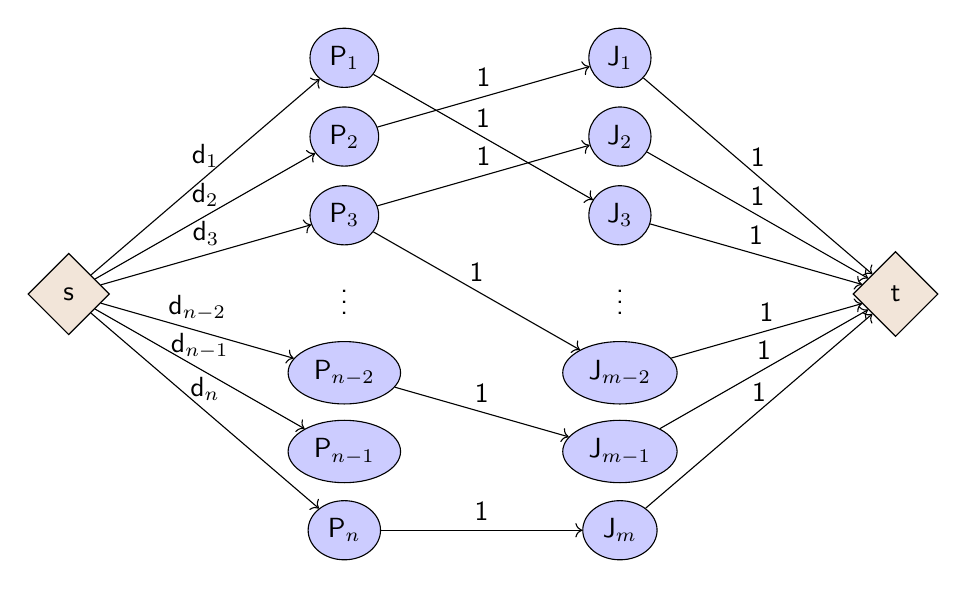
\begin{tikzpicture}[main/.style = {draw, circle}] 
    \node[sink] (1) {s};
    \node (2) [right of=1, node distance=3.5cm]  {$\vdots$};
    \node[cloud] (3) [above of=2,node distance=1cm] {P$_3$};
    \node[cloud] (9) [right of=3,node distance=3.5cm] {J$_3$};
    \node[cloud] (4) [above of=3,node distance=1cm] {P$_2$};
    \node[cloud] (10) [right of=4,node distance=3.5cm] {J$_2$};
    \node[cloud] (5) [below of=2,node distance=1cm] {P$_{n-2}$};
    \node[cloud] (11) [right of=5,node distance=3.5cm] {J$_{m-2}$};
    \node[cloud] (6) [below of=5,node distance=1cm] {P$_{n-1}$};
    \node[cloud] (12) [right of=6,node distance=3.5cm] {J$_{m-1}$};
    \node[cloud] (7) [below of=6,node distance=1cm] {P$_n$};
    \node[cloud] (13) [right of=7,node distance=3.5cm] {J$_m$};
    \node[cloud] (8) [above of=4,node distance=1cm] {P$_1$};
    \node[cloud] (14) [right of=8,node distance=3.5cm] {J$_1$};
    \node (15) [right of=2, node distance=3.5cm]  {$\vdots$};
    \node[sink] (16) [right of=15,node distance=3.5cm] {t};
    %\draw[->] (1) -- node[midway,above]{$\infty$} (2);
    \draw[->] (1) -- node[midway,above]{d$_3$} (3);
    \draw[->] (1) -- node[midway,above]{d$_2$} (4);
    \draw[->] (1) -- node[midway,above]{d$_{n-2}$} (5);
    \draw[->] (1) -- node[midway,above]{d$_{n-1}$} (6);
    \draw[->] (1) -- node[midway,above]{d$_n$} (7);
    \draw[->] (1) -- node[midway,above]{d$_1$} (8);
    \draw[<-] (16) -- node[midway,above]{1} (9);
    \draw[<-] (16) -- node[midway,above]{1} (10);
    \draw[<-] (16) -- node[midway,above]{1} (11);
    \draw[<-] (16) -- node[midway,above]{1} (12);
    \draw[<-] (16) -- node[midway,above]{1} (13);
    \draw[<-] (16) -- node[midway,above]{1} (14);
    \draw[->] (3) -- node[midway,above]{1} (11);
    \draw[->] (4) -- node[midway,above]{1} (14);
    \draw[->] (5) -- node[midway,above]{1} (12);
    \draw[->] (3) -- node[midway,above]{1} (10);
    \draw[->] (7) -- node[midway,above]{1} (13);
    \draw[->] (8) -- node[midway,above]{1} (9);
 \end{tikzpicture}
 \end{center}
 For Some \textbf{integer} valued flow in the Graph \textbf{G} we have the following a person is assigned a Job if \textbf{f}(P$_i$,J$_j$) = 1 
 \begin{enumerate}
     \item Such a Flow assignment has a person P$_i$ getting assigned at most d$_i$ Jobs.
     \begin{itemize}
         \item This is due to Flow conservation at Person nodes
         \item Therefore at most d$_i$ Job can be assigned since there is only incoming edge with capacity d$_i$ which means at most d$_i$ outgoing edges with capacity 1.
         \item Since \textbf{f}(e) $\leq$ \textbf{c}(e), The above claim holds true.
     \end{itemize}
     \item Such a Flow assignment has a person getting assigned the Job he is willing to do.
     \begin{itemize}
         \item This is due to the construction of the graph.
         \item Edges are present in the main graph if and only if a person is willing to do the Job
     \end{itemize}
     \item Such a Flow Assignment has \textbf{f}(J$_j$,t) = 1 if and only if J$_j$ is assigned.
     \begin{itemize}
         \item This is due to Flow conservation at Job Nodes
         \item If a Job is assigned to a person P$_i$ that means there is an incoming edge with \textbf{f}(P$_i$,J$_j$) = 1
         \item Since only one outgoing edge its flow value \textbf{f}(J$_j$,t) must also be 1 and this job is not assigned to any other person except the person P$_i$
     \end{itemize}
 \end{enumerate}
 \boxed{\text{\large\textbf{Lemma} : \textbf{G} has a flow of value $n$ if and only if all the jobs are assigned}}  \\
    \vspace*{0em}\\
 \textbf{Proof} : Suppose \textbf{G} has a flow of size n. ($\implies$)\vspace{0.5em}\\
 \rule[0.5mm]{1.1cm}{0pt} This means that \textbf{f}(j,t) = 1 for j $\in$ \textbf{E}$_t$\\
 \rule[0.5cm]{1.1cm}{0pt} Hence All Jobs are assigned.\\
 \rule[0.5cm]{1.1cm}{0pt} Suppose all Jobs are not assigned.($\impliedby$)\\
 \rule[0.5cm]{1.1cm}{0pt} This means that there is some Job j that is not assigned\\
 \rule[0.5cm]{1.1cm}{0pt} Hence \textbf{f}(j,t) = 0  which means $|\mathbf{f}|$ = \textbf{f}$^\gets$(t) = $\sum_1^n$ \textbf{f}(j,t) $<$ n\\
 \subsection*{c)}
 We Construct the Graph \textbf{G} by giving its  vertices \textbf{V}, edges \textbf{E}, and capacities \textbf{c} : \textbf{E} $\rightarrow$ $\mathbb{N}$\\
 \rule[0.5cm]{2cm}{0pt} Let \textbf{P} be the set of all Persons and \textbf{J} be the set of all Jobs\\
 \rule[0.5mm]{2cm}{0pt} \textbf{V} = \{s\} $\cup$ \{t\} $\cup$ \{P$_i$ $|$ i $\in$ \textbf{P}\} $\cup$ \{Q$_i$ $|$ i $\in$ \textbf{P}\} $\cup$ \{J$_j$ $|$ j $\in$ \textbf{J}\} \\
 \vspace*{0em}\\
 \rule[0.5mm]{2cm}{0pt} Let \textbf{T} be all those pairs (i,j) where ith person is willing to do jth Job.\\
 \rule[0.5mm]{2cm}{0pt} \textbf{E} = \textbf{E$_{s}$} $\cup$ \textbf{E$_{pq}$}$\cup$ \textbf{E$_{mb}$} $\cup$ \textbf{E$_{m}$} $\cup$  \textbf{E$_{t}$} where\\
 \begin{equation*}
     \mathbf{E}_s = \{(s,P_i)\  |\  i \in \mathbf{P}\} 
 \end{equation*}
 \begin{equation*}
     \mathbf{E}_{pq} = \{(P_i,Q_i)\  | \ i \in \mathbf{P} \}
 \end{equation*}
 \begin{equation*}
     \mathbf{E}_{mb} = \{(Q_i,J_j)\  | \ (i,j) \in \mathbf{T} \text{ and j is a boring job} \}
 \end{equation*}
 \begin{equation*}
     \mathbf{E}_m = \{(P_i,J_j)\  | \ (i,j) \in \mathbf{T} \text{ and j is not a boring job} \}
 \end{equation*}
 \begin{equation*}
     \mathbf{E}_t = \{(J_j,t)\ |\  j \in \mathbf{J}\}
 \end{equation*}
  \rule[0.5mm]{2cm}{0pt} The map \textbf{c} is defined as follows \\
   \[   
    \textbf{c(e)} = 
         \begin{cases}
           d_i &\quad\text{if }(s,P_i) \in \mathbf{E}_s\\
           b_i &\quad\text{if }(P_i,Q_i) \in \mathbf{E}_{pq}\\
           1 &\quad\text{if e} \in \mathbf{E}_{mb}\\
           1 &\quad\text{if e} \in \mathbf{E}_m\\
           1 &\quad\text{if e} \in \mathbf{E}_t\\
         \end{cases}
    \]
 For example, one such graph would be as follows where boring Jobs are J$_1$,J$_2$,J$_{m-2}$ and J$_m$, and interesting Jobs are J$_3$,J$_{m-1}$.\\
 \begin{center}
 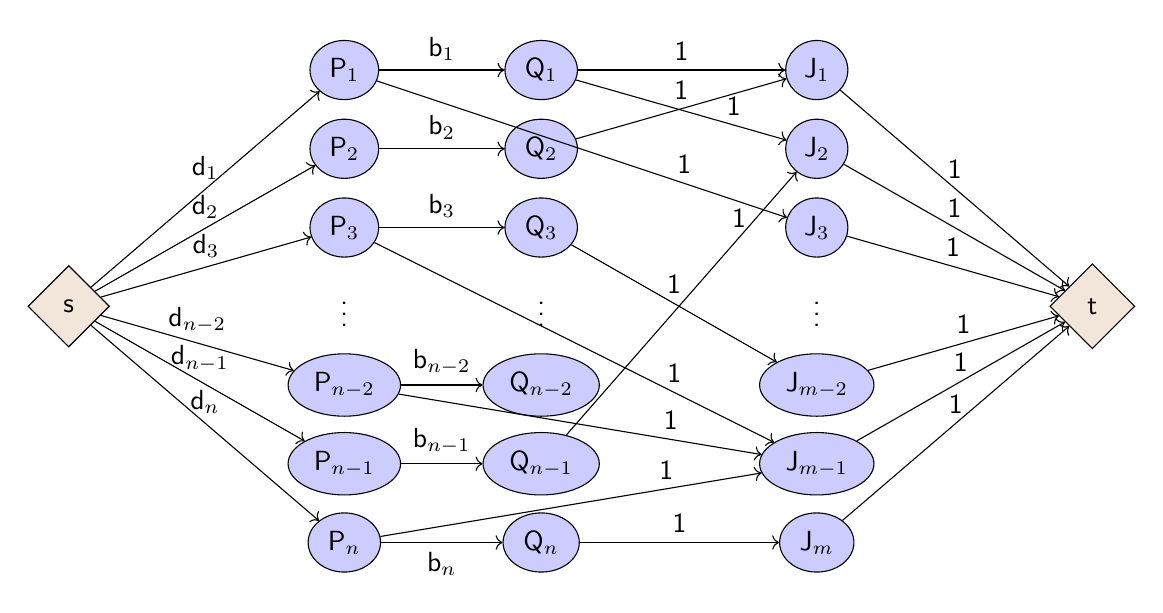
\begin{tikzpicture}[main/.style = {draw, circle}] 
    \node[sink] (1) {s};
    \node (2) [right of=1, node distance=3.5cm]  {$\vdots$};
    \node[cloud] (3) [above of=2,node distance=1cm] {P$_3$};
    \node[cloud] (9) [right of=3,node distance=6cm] {J$_3$};
    \node[cloud] (4) [above of=3,node distance=1cm] {P$_2$};
    \node[cloud] (10) [right of=4,node distance=6cm] {J$_2$};
    \node[cloud] (5) [below of=2,node distance=1cm] {P$_{n-2}$};
    \node[cloud] (11) [right of=5,node distance=6cm] {J$_{m-2}$};
    \node[cloud] (6) [below of=5,node distance=1cm] {P$_{n-1}$};
    \node[cloud] (12) [right of=6,node distance=6cm] {J$_{m-1}$};
    \node[cloud] (7) [below of=6,node distance=1cm] {P$_n$};
    \node[cloud] (13) [right of=7,node distance=6cm] {J$_m$};
    \node[cloud] (8) [above of=4,node distance=1cm] {P$_1$};
    \node[cloud] (14) [right of=8,node distance=6cm] {J$_1$};
    \node (15) [right of=2, node distance=6cm]  {$\vdots$};
    \node[cloud] (17) [right of=3,node distance=2.5cm] {Q$_3$};
    \node[cloud] (18) [right of=4,node distance=2.5cm] {Q$_2$};
    \node[cloud] (19) [right of=5,node distance=2.5cm] {Q$_{n-2}$};
    \node[cloud] (20) [right of=6,node distance=2.5cm] {Q$_{n-1}$};
    \node[cloud] (21) [right of=7,node distance=2.5cm] {Q$_n$};
    \node[cloud] (22) [right of=8,node distance=2.5cm] {Q$_1$};
    \node (23) [right of=2, node distance=2.5cm]  {$\vdots$};
    \node[sink] (16) [right of=15,node distance=3.5cm] {t};
    %\draw[->] (1) -- node[midway,above]{$\infty$} (2);
    \draw[->] (1) -- node[midway,above]{d$_3$} (3); 
    \draw[->] (1) -- node[midway,above]{d$_2$} (4);
    \draw[->] (1) -- node[midway,above]{d$_{n-2}$} (5);
    \draw[->] (1) -- node[midway,above]{d$_{n-1}$} (6);
    \draw[->] (1) -- node[midway,above]{d$_n$} (7);
    \draw[->] (1) -- node[midway,above]{d$_1$} (8);
    \draw[<-] (17) -- node[midway,above]{b$_3$} (3); 
    \draw[<-] (18) -- node[midway,above]{b$_2$} (4);
    \draw[<-] (19) -- node[midway,above]{b$_{n-2}$} (5);
    \draw[<-] (20) -- node[midway,above]{b$_{n-1}$} (6);
    \draw[<-] (21) -- node[midway,below]{b$_n$} (7);
    \draw[<-] (22) -- node[midway,above]{b$_1$} (8);
    \draw[<-] (16) -- node[midway,above]{1} (9);
    \draw[<-] (16) -- node[midway,above]{1} (10);
    \draw[<-] (16) -- node[midway,above]{1} (11);
    \draw[<-] (16) -- node[midway,above]{1} (12);
    \draw[<-] (16) -- node[midway,above]{1} (13);
    \draw[<-] (16) -- node[midway,above]{1} (14);
    \draw[->] (17) -- node[midway,above]{1} (11);
    \draw[->] (18) -- node[midway,above]{1} (14);
    \draw[->] (5) -- node[near end,above]{1} (12);
    \draw[->] (20) -- node[near end,above]{1} (10);
    \draw[->] (21) -- node[midway,above]{1} (13);
    \draw[->] (8) -- node[near end,above]{1} (9);
    \draw[->] (22) -- node[midway,above]{1} (14);
    \draw[->] (7) -- node[near end,above]{1}(12);
    \draw[->] (3) -- node[near end,above]{1} (12);
    \draw[->] (22) -- node[near end,above]{1} (10);
 \end{tikzpicture}
 \end{center}
 For Some \textbf{integer} valued flow in the Graph \textbf{G} we have the following a person i is assigned a Job j if \textbf{f}(P$_i$,J$_j$) = 1 or \textbf{f}(Q$_i$,J$_j$) = 1.
 \begin{enumerate}
     \item Such a Flow assignment has a person i doing at most b$_i$ boring jobs
     \begin{itemize}
         \item This is due to Flow conservation at node Q$_i$.
         \item Since the node Q$_i$ has edges to Jobs J$_j$ if and only if J$_j$ is a boring Job
         \item Therefore \textbf{f}$^\rightarrow$(Q$_i$) = B(i) where B(i) is the number of boring jobs done by person i.
         \item Hence a person does at most b$_i$ boring jobs.
         \item Since \textbf{f}(e) $\leq$ \textbf{c}(e), The above claim holds true.
     \end{itemize}
     \item Such a Flow assignment has a person i getting assigned at most d$_i$ Jobs.
     \begin{itemize}
         \item This is due to Flow conservation at set I = \{P$_i$,Q$_i$\}.
         \item \textbf{f}$^\gets$(I) = \textbf{f}$^\rightarrow$(I) $\implies$ \textbf{f}$^\gets$(P$_i$) + \textbf{f}$^\gets$(Q$_i$) = \textbf{f}$^\rightarrow$(P$_i$) + \textbf{f}$^\rightarrow$(Q$_i$)
         \item \textbf{f}$^\rightarrow$(P$_i$) = \textbf{f}$^\rightarrow$(Q$_i$) + n(i) where n(i) is the number of interesting jobs done by person i.
         \item Hence \textbf{f}$^\gets$(P$_i$) = n(i) + B(i) = T(i) where T(i) is total number of jobs done by person i.
         \item Hence we have a person doing at most d$_i$ jobs
         \item Since \textbf{f}(e) $\leq$ \textbf{c}(e), The above claim holds true.
     \end{itemize}
     \item Such a Flow assignment has a person getting assigned the Job he is willing to do.
     \begin{itemize}
         \item This is due to the construction of the graph.
         \item Edges are present in the main graph if and only if a person is willing to do the Job irrespective of boring or interesting Jobs.
         \item If the person is willing to do Job J$_j$ which is boring then edge (Q$_i$,J$_j$) is present if it is not boring then edge (P$_i$,J$_j$) is present.
      \end{itemize}
     \item Such a Flow Assignment doesn't have both \textbf{f}(P$_i$,J$_j$) = 1 and \textbf{f}(Q$_i$,J$_j$) = 1.
     \begin{itemize}
         \item If \textbf{f}(P$_i$,J$_j$) = 1 then edge (P$_i$,J$_j$) which means J$_j$ is an interesting Job and hence no Q$_k$ is connected to it according to the definition of graph \textbf{G}.
         \item If \textbf{f}(Q$_i$,J$_j$) = 1 then edge (Q$_i$,J$_j$) which means J$_j$ is an boring Job and hence no P$_k$ is connected to it according to the definition of the graph \textbf{G}.
     \end{itemize}
     \item Such a Flow Assignment has \textbf{f}(J$_j$,t) = 1 if and only if J$_j$ is assigned.
     \begin{itemize}
         \item This is due to Flow conservation at Job Nodes
         \item If a Job is assigned to a person P$_i$ that means there is an incoming edge with \textbf{f}(P$_i$,J$_j$) = 1 or \textbf{f}(Q$_i$,J$_j$) = 1
         \item Since only one outgoing edge its flow value \textbf{f}(J$_j$,t) must also be 1 and this job is not assigned to any other person except the person i.
         \item Suppose \textbf{f}(P$_i$,J$_j$) = 1 or \textbf{f}(Q$_i$,J$_j$) = 1 which means J$_j$ was assigned.
     \end{itemize}
 \end{enumerate}
 \boxed{\text{\large\textbf{Lemma} : \textbf{G} has a flow of value $n$ if and only if all the jobs are assigned}}  \\
    \vspace*{0em}\\
 \textbf{Proof} : Suppose \textbf{G} has a flow of size n. ($\implies$)\vspace{0.5em}\\
 \rule[0.5mm]{1.1cm}{0pt} This means that \textbf{f}(j,t) = 1 for j $\in$ \textbf{E}$_t$\\
 \rule[0.5cm]{1.1cm}{0pt} Hence All Jobs are assigned.\\
 \rule[0.5cm]{1.1cm}{0pt} Suppose all Jobs are not assigned.($\impliedby$)\\
 \rule[0.5cm]{1.1cm}{0pt} This means that there is some Job j that is not assigned\\
 \rule[0.5cm]{1.1cm}{0pt} Hence \textbf{f}(j,t) = 0  which means $|\mathbf{f}|$ = \textbf{f}$^\gets$(t) = $\sum_1^n$ \textbf{f}(j,t) $<$ n\\
 \vspace*{0.5em}\\
 If the problem was feasible then max flow in the graph network would give the required assignment of Jobs.
 \subsection*{d)}We Construct the Graph \textbf{G} by giving its  vertices \textbf{V}, edges \textbf{E}, and capacities \textbf{c} : \textbf{E} $\rightarrow$ $\mathbb{N}$\\
 \rule[0.5cm]{2cm}{0pt} Let \textbf{P} be the set of all Persons and \textbf{J} be the set of all Jobs\\
 \rule[0.5mm]{2cm}{0pt} \textbf{V} = \{s\} $\cup$ \{t\} $\cup$ \{P$_i$ $|$ i $\in$ \textbf{P}\} $\cup$ \{Q$_i$ $|$ i $\in$ \textbf{P}\} $\cup$ \{J$_j$ $|$ j $\in$ \textbf{J}\} \\
 \vspace*{0em}\\
 \rule[0.5mm]{2cm}{0pt} Let \textbf{T} be all those pairs (i,j) where ith person is willing to do jth Job.\\
 \rule[0.5mm]{2cm}{0pt} \textbf{E} = \textbf{E$_{s}$} $\cup$ \textbf{E$_{pq}$}$\cup$ \textbf{E$_{mb}$} $\cup$ \textbf{E$_{m}$} $\cup$  \textbf{E$_{t}$} where\\
 \begin{equation*}
     \mathbf{E}_s = \{(s,P_i)\  |\  i \in \mathbf{P}\} 
 \end{equation*}
 \begin{equation*}
     \mathbf{E}_{pq} = \{(P_i,Q_i)\  | \ i \in \mathbf{P} \}
 \end{equation*}
 \begin{equation*}
     \mathbf{E}_{mb} = \{(Q_i,J_j)\  | \ (i,j) \in \mathbf{T} \text{ and j is a boring job for person i} \}
 \end{equation*}
 \begin{equation*}
     \mathbf{E}_m = \{(P_i,J_j)\  | \ (i,j) \in \mathbf{T} \text{ and j is not a boring job for person i} \}
 \end{equation*}
 \begin{equation*}
     \mathbf{E}_t = \{(J_j,t)\ |\  j \in \mathbf{J}\}
 \end{equation*}
  \rule[0.5mm]{2cm}{0pt} The map \textbf{c} is defined as follows \\
   \[   
    \textbf{c(e)} = 
         \begin{cases}
           d_i &\quad\text{if }(s,P_i) \in \mathbf{E}_s\\
           b_i &\quad\text{if }(P_i,Q_i) \in \mathbf{E}_{pq}\\
           1 &\quad\text{if e} \in \mathbf{E}_{mb}\\
           1 &\quad\text{if e} \in \mathbf{E}_m\\
           1 &\quad\text{if e} \in \mathbf{E}_t\\
         \end{cases}
    \]
 For example, one such graph would be as follows where
 \begin{itemize}
    \item P$_1$ feels J$_2$ as interesting and J$_1$ as boring job of the willing jobs.
    \item P$_2$ feels J$_1$ as interesting and J$_3$ as boring job of the willing jobs.
    \item P$_3$ feels J$_{m-2}$ as interesting job.
    \item P$_{n-2}$ feels J$_{m-2}$ as boring job.
    \item P$_{n-1}$ feels J$_{m-1}$,J$_{m-1}$ as boring and J$_m$ as interesting jobs.
    \item P$_n$ feels J$_m$ as boring Job.
 \end{itemize}
 \begin{center}
 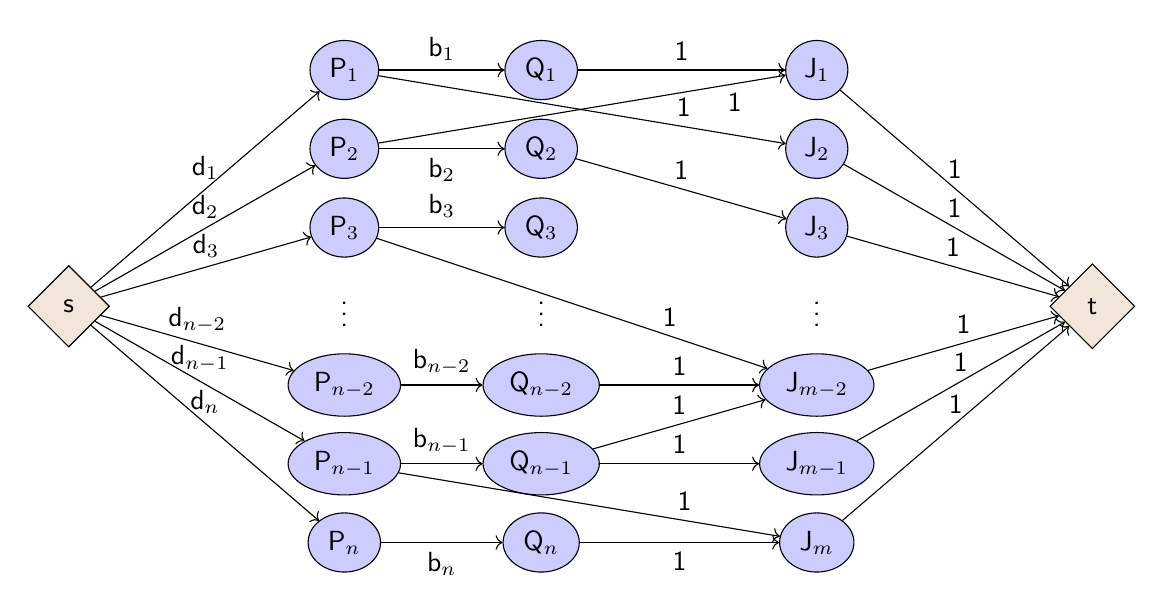
\begin{tikzpicture}[main/.style = {draw, circle}] 
    \node[sink] (1) {s};
    \node (2) [right of=1, node distance=3.5cm]  {$\vdots$};
    \node[cloud] (3) [above of=2,node distance=1cm] {P$_3$};
    \node[cloud] (9) [right of=3,node distance=6cm] {J$_3$};
    \node[cloud] (4) [above of=3,node distance=1cm] {P$_2$};
    \node[cloud] (10) [right of=4,node distance=6cm] {J$_2$};
    \node[cloud] (5) [below of=2,node distance=1cm] {P$_{n-2}$};
    \node[cloud] (11) [right of=5,node distance=6cm] {J$_{m-2}$};
    \node[cloud] (6) [below of=5,node distance=1cm] {P$_{n-1}$};
    \node[cloud] (12) [right of=6,node distance=6cm] {J$_{m-1}$};
    \node[cloud] (7) [below of=6,node distance=1cm] {P$_n$};
    \node[cloud] (13) [right of=7,node distance=6cm] {J$_m$};
    \node[cloud] (8) [above of=4,node distance=1cm] {P$_1$};
    \node[cloud] (14) [right of=8,node distance=6cm] {J$_1$};
    \node (15) [right of=2, node distance=6cm]  {$\vdots$};
    \node[cloud] (17) [right of=3,node distance=2.5cm] {Q$_3$};
    \node[cloud] (18) [right of=4,node distance=2.5cm] {Q$_2$};
    \node[cloud] (19) [right of=5,node distance=2.5cm] {Q$_{n-2}$};
    \node[cloud] (20) [right of=6,node distance=2.5cm] {Q$_{n-1}$};
    \node[cloud] (21) [right of=7,node distance=2.5cm] {Q$_n$};
    \node[cloud] (22) [right of=8,node distance=2.5cm] {Q$_1$};
    \node (23) [right of=2, node distance=2.5cm]  {$\vdots$};
    \node[sink] (16) [right of=15,node distance=3.5cm] {t};
    %\draw[->] (1) -- node[midway,above]{$\infty$} (2);
    \draw[->] (1) -- node[midway,above]{d$_3$} (3); 
    \draw[->] (1) -- node[midway,above]{d$_2$} (4);
    \draw[->] (1) -- node[midway,above]{d$_{n-2}$} (5);
    \draw[->] (1) -- node[midway,above]{d$_{n-1}$} (6);
    \draw[->] (1) -- node[midway,above]{d$_n$} (7);
    \draw[->] (1) -- node[midway,above]{d$_1$} (8);
    \draw[<-] (17) -- node[midway,above]{b$_3$} (3); 
    \draw[<-] (18) -- node[midway,below]{b$_2$} (4);
    \draw[<-] (19) -- node[midway,above]{b$_{n-2}$} (5);
    \draw[<-] (20) -- node[midway,above]{b$_{n-1}$} (6);
    \draw[<-] (21) -- node[midway,below]{b$_n$} (7);
    \draw[<-] (22) -- node[midway,above]{b$_1$} (8);
    \draw[<-] (16) -- node[midway,above]{1} (9);
    \draw[<-] (16) -- node[midway,above]{1} (10);
    \draw[<-] (16) -- node[midway,above]{1} (11);
    \draw[<-] (16) -- node[midway,above]{1} (12);
    \draw[<-] (16) -- node[midway,above]{1} (13);
    \draw[<-] (16) -- node[midway,above]{1} (14);
    \draw[->] (8) -- node[near end,above]{1} (10);
    \draw[->] (22) -- node[midway,above]{1} (14);
    \draw[->] (4) -- node[very near end,below]{1} (14);
    \draw[->] (18) -- node[midway,above]{1} (9);
    \draw[->] (3) -- node[near end,above]{1} (11);
    \draw[->] (19) -- node[midway,above]{1} (11);
    \draw[->] (20) -- node[midway,above]{1} (11);
    \draw[->] (20) -- node[midway,above]{1} (12);
    \draw[->] (6) -- node[near end,above]{1} (13);
    \draw[->] (21) -- node[midway,below]{1} (13);
 \end{tikzpicture}
 \end{center}
 For Some \textbf{integer} valued flow in the Graph \textbf{G} we have the following a person i is assigned a Job j if \textbf{f}(P$_i$,J$_j$) = 1 or \textbf{f}(Q$_i$,J$_j$) = 1.
 \begin{enumerate}
     \item Such a Flow assignment has a person i doing at most b$_i$ jobs which he feels boring.
     \begin{itemize}
         \item This is due to Flow conservation at node Q$_i$.
         \item Since the node Q$_i$ has edges to Jobs J$_j$ if and only if person i feels that  J$_j$ is a boring Job.
         \item Therefore \textbf{f}$^\rightarrow$(Q$_i$) = B(i) where B(i) is the number of  jobs assigned to person i which he feels boring.
         \item Hence a person does at most b$_i$ jobs which he feels boring 
         \item Since \textbf{f}(e) $\leq$ \textbf{c}(e), The above claim holds true.
     \end{itemize}
     \item Such a Flow assignment has a person i getting assigned at most d$_i$ Jobs.
     \begin{itemize}
         \item This is due to Flow conservation at set I = \{P$_i$,Q$_i$\}.
         \item \textbf{f}$^\gets$(I) = \textbf{f}$^\rightarrow$(I) $\implies$ \textbf{f}$^\gets$(P$_i$) + \textbf{f}$^\gets$(Q$_i$) = \textbf{f}$^\rightarrow$(P$_i$) + \textbf{f}$^\rightarrow$(Q$_i$)
         \item \textbf{f}$^\rightarrow$(P$_i$) = \textbf{f}$^\rightarrow$(Q$_i$) + n(i) where n(i) is the number of jobs done by person i which he feels interesting.
         \item Hence \textbf{f}$^\gets$(P$_i$) = n(i) + B(i) = T(i) where T(i) is total number of jobs done by person i.
         \item Hence we have a person doing at most d$_i$ jobs
         \item Since \textbf{f}(e) $\leq$ \textbf{c}(e), The above claim holds true.
     \end{itemize}
     \item Such a Flow assignment has a person getting assigned the Job he is willing to do.
     \begin{itemize}
         \item This is due to the construction of the graph.
         \item Edges are present in the main graph if and only if a person is willing to do the Job irrespective of boring or interesting Jobs.
         \item If the person is willing to do Job J$_j$ which he feels boring then edge (Q$_i$,J$_j$) is present if he feels interesting then edge (P$_i$,J$_j$) is present.
      \end{itemize}
     \item Such a Flow Assignment doesn't have both \textbf{f}(P$_i$,J$_j$) = 1 and \textbf{f}(Q$_i$,J$_j$) = 1.
     \begin{itemize}
         \item If \textbf{f}(P$_i$,J$_j$) = 1 then edge (P$_i$,J$_j$) which means J$_j$ is an interesting Job according to person i and hence Q$_i$ is not connected to it.
         \item If \textbf{f}(Q$_i$,J$_j$) = 1 then edge (Q$_i$,J$_j$) which means J$_j$ is an boring Job according to person i and hence P$_i$ is not connected to it.
     \end{itemize}
     \item Such a Flow Assignment has \textbf{f}(J$_j$,t) = 1 if and only if J$_j$ is assigned.
     \begin{itemize}
         \item This is due to Flow conservation at Job Nodes
         \item If a Job is assigned to a person P$_i$ that means there is an incoming edge with \textbf{f}(P$_i$,J$_j$) = 1 or \textbf{f}(Q$_i$,J$_j$) = 1
         \item Since only one outgoing edge its flow value \textbf{f}(J$_j$,t) must also be 1 and this job is not assigned to any other person except the person i.
         \item Suppose \textbf{f}(P$_i$,J$_j$) = 1 or \textbf{f}(Q$_i$,J$_j$) = 1 which means J$_j$ was assigned.
     \end{itemize}
 \end{enumerate}
 \boxed{\text{\large\textbf{Lemma} : \textbf{G} has a flow of value $n$ if and only if all the jobs are assigned}}  \\
    \vspace*{0em}\\
 \textbf{Proof} : Suppose \textbf{G} has a flow of size n. ($\implies$)\vspace{0.5em}\\
 \rule[0.5mm]{1.1cm}{0pt} This means that \textbf{f}(j,t) = 1 for j $\in$ \textbf{E}$_t$\\
 \rule[0.5cm]{1.1cm}{0pt} Hence All Jobs are assigned.\\
 \rule[0.5cm]{1.1cm}{0pt} Suppose all Jobs are not assigned.($\impliedby$)\\
 \rule[0.5cm]{1.1cm}{0pt} This means that there is some Job j that is not assigned\\
 \rule[0.5cm]{1.1cm}{0pt} Hence \textbf{f}(j,t) = 0  which means $|\mathbf{f}|$ = \textbf{f}$^\gets$(t) = $\sum_1^n$ \textbf{f}(j,t) $<$ n\\
 \vspace*{0.5em}\\
 If the problem was feasible then max flow in the graph network would give the required assignment of Jobs.
 \section*{Question 2}
 \subsection*{a)}
 Let $G'(V,E')$ be transitive closure of $G(V,E)$ i.e $\forall(x,y),(y,z)\in E, (x,z) \in E'$\\
 For solving this question we will show that\\
 Minimum number of path such that each vertices is in at least one path in $G$ = Minimum number of path such that each vertices is in exactly one path in $G'$\\
 
 \textbf{Claim 1:}
 If there is a minimum path cover $P'$ of $G'$ such that each vertices is in exactly one path there exist another path cover $P$ of $G$ such that each vertices is in at least one path with $|P| = |P'|$\\
 
 \textbf{Proof:}\\
 For every path $p'$ in set $P'$ we add a path $p$ in $P$.\\
 We construct $p$ from $p'$ in following way:
 \begin{enumerate}
     \item  If edge $(x,y) \in E$ we add it in p.
     \item   If edge $(x,y) \not\in E$ we add path $x \rightarrow y$ to $p$ as $G'$ is transitive closure of $G$ there exist a path $x \rightarrow y$.
 \end{enumerate}

 Also by construction of $p$ we can see that each vertices $x \in p'$ also belongs to $p$ and hence $P$ is a path cover.\\
 
 \textbf{Claim 2:}
 If there exist a minimum path cover $P$ of $G$ such that each vertices is in at least one path there exist other path cover $P'$ of $G'$ such that each vertices is in exactly one path with $|P| = |P'|$\\
 
\textbf{Proof:}\\
For every path $p$ in set $P$ we add a path $p'$ in $P'$.\\
 We construct $p'$ from $p$ in following way:
 \begin{enumerate}
     \item If the vertices $x$ is not already in any path in $P'$ we add x to $p'$
     \item If the vertices $x$ is already present in a path in $P'$ we don't add it. If the vertices is at start or end of path its removal give us one path only. If it is in middle of path say $yxz$ then $yz$ is an edge in $G'$ and hence even after removal of vertices $x$ we get one path only.
 \end{enumerate}
 We also note that each path $p$ contains at least one unique node and hence no path $p'$ will be empty.\\
 
 Also by construction we can see that all the vertices covered till path $p_i$ is also covered till $p'_i$\\
 
 Now by using above two claim we can see that\\
  Minimum number of path such that each vertices is in at least one path in $G$ = Minimum number of path such that each vertices is in exactly one path in $G'$\\
  
  Now minimum number of path such that each vertices is in exactly one path in $G'$ is solved in \textbf{b)}
 \subsection*{b)}
 Given graph $G = (V, E)\,, |V| = n $ we construct another bipartite graph $G' = (V_{out}\cup V_{in} ,E')$ where 
 \begin{enumerate}
     \item $V_{out}$ = $\{v_{out} \;| v \,\in\, V\: \land \: v$ has positive out-degree\}
     \item  $V_{in}$ = $\{v_{in} | v\;\in\; V\: \land \: v $ has positive indegree\}
     \item \{ $(u_{out},v_{in})\: \in V_{out}\times V_{in}\: | (u,v) \: in \: E\}$
 \end{enumerate}
 
 Then running the maximum flow algorithm on $G'$ with capacity of each edge 1 gives the minimum path cover of $G$ where edge $(u,v)$ is in a path of path cover if $(u_{out},v_{in})$ has a flow of 1.\\
 
 We will prove the above claim using flowing observations:-
 \begin{enumerate}
     \item  No vertex appears twice in path cover.
     
       Suppose vertices x occurs twice then there are two cases
       \begin{itemize}
           \item there are two edges $(x_{out}, y_{in}), (x_{out}, z_{in}) $ such that $x\;\neq y\;\neq z$ in flow with flow value 1 but $x_{out}$ can have maximum incoming flow of 1 as $(s,x_{out})$ has capacity of 1. Hence it violates our conservation law and our assumption is incorrect
           \item Similarly we can't have flow value of 1 for edges $(y_{out},x_{in}),(z_{out},x_{in})$ as outgoing edge $(x_{in}, t)$ has capacity of 1
         \end{itemize} 
         
    \item
    Each vertices is covered. Suppose a vertices $x$ has no  edge of form $(x_{out},y_{in})$ or $(z_{out},x_{in})$ with flow value 1 then it itself forms path.  
    \item
    Suppose the algorithm yields path cover with k paths then there are n-k edges which is equal to the the value of maximum flow as for each edge in path cover there is an edge $(x_{out}, y_{in})$ with flow value 1 and for each such edge there is value of flow of edge $(s, x_{out}) = 1$.
    \item
    Given a vertices disjoint path cover we can recover flow by assigning edges $(s,x_{out})\,, (x_{out}, y_{in}),\,(y_{in},t)$ flow value of 1 for each edge $(x,y)$ in path cover. The above assignment respects conservation and capacity.
    \item
    Let the maximum flow algorithm gives maximum flow value of $n-k$ and hence number of paths $k$.\\
    Suppose it is not minimum hence there exist a minimum path cover with cardinality less than $k$ which implies we can construct a flow of $G'$ with maximm-flow value greater than $n-k$ but it contradicts our assumption that maximum flow value of graph $G'$ is $n-k$
       
      
 \end{enumerate}
 So the minimum number of paths required is n - $MaxFlow(G')$ 
 \subsection*{c)}
 Let $G \,=\, (V, \, E)$. We construct $G' = (V', \, E')$ such that\\
 \begin{enumerate}
     \item
     $V'\; = \; \{xy | (x,y)\in E\}$
     \item
     $E' \; = \; \{(xy,yz) | (x,y) , (y, z)\in E\}$
     
 \end{enumerate}
 
 We will show that\\ minimum number of edge-disjoint  paths required to cover each edge  of graph $G$ = minimum number of vertex-disjoint paths required to cover each vertices of graph $G'$ using following observations:-
 \begin{enumerate}\item
 A minimum path cover $P$ of graph of $G$ can be transformed into path cover $P'$ of $G'$ satisfying their respective properties with $|P| = |P'|$.\\
 \begin{itemize}
     \item 
 
 We note that each path of $P$ has at least one edge.
 \item
 We can  construct $P'$ from $P = x_0,x_1,x_2,.....,x_n$ as $x_0x_1, x_1x_2,......,x_{n-1}x_n$ 
 \item
 Since every edge is covered in $P$ and every every edge of $G$ corresponds to a vertices in $G'$ every vertices is covered in $G'$
 \end{itemize}
 \item
 Similarly a minimum  path cover of $G'$ can be transformed into path cover of $G$ satisfying their respective properties with $|P| = |P'|$ as edge of $G$ to vertices of $G'$ is bijection.
 \end{enumerate}
 
 Using above two observations we have showed our claim.\\
 Now we can use  the result we obtained in part $b)$ for graph $G'$ to obtain the result for graph $G$
 \subsection*{d)}
 In part $b)$ we noted that for each edge in path cover maximum flow value increased by one. Since a path covering $n$ vertices has $n-1$ edge it contributes $n-1$ to maximum flow and the number of path will increase by $n-(n-1) \,=\, 1$.\\
 Now consider a cycle with $n$ vertices present in a graph it contains $n$ edges. So maximum flow value corresponding to this path may increase by a value of $n$ contributing $n-n\,=\,0$ to number of paths and hence giving incorrect result.\\
 For example we consider a simple cyclic directed graph consisting of 3 nodes.\\
 \begin{center}
 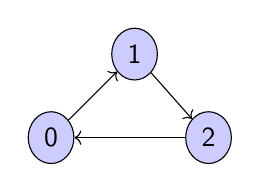
\begin{tikzpicture}
    \node[cloud] (1) {0};
    \node[cloud] (2) [above right of=1,node distance=1.5cm] {1};
    \node[cloud] (3) [right of=1,node distance=2cm] {2};
    \draw[->] (1) -- (2);
    \draw[->] (2) -- (3);
    \draw[->] (3) -- (1);
 \end{tikzpicture}
 \end{center}
 Making G' as specified in b) and running max flow algorithm gives 
 \begin{center}
 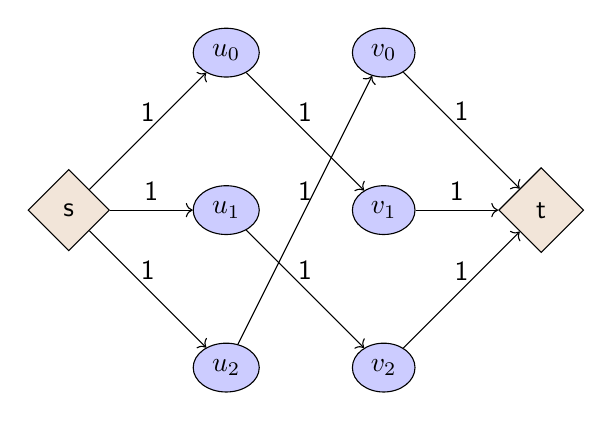
\begin{tikzpicture}
    \node[sink] (1) {s};
    \node[cloud] (2) [right of=1,node distance=2cm] {$u_1$};
    \node[cloud] (3) [above of=2,node distance=2cm] {$u_0$};
    \node[cloud] (4) [below of=2,node distance=2cm] {$u_2$};
    \node[cloud] (5) [right of=2,node distance=2cm] {$v_1$};
    \node[cloud] (6) [right of=3,node distance=2cm] {$v_0$};
    \node[cloud] (7) [right of=4,node distance=2cm] {$v_2$};
    \node[sink] (8) [right of=5,node distance=2cm] {t};
    \draw[->] (1) -- node[midway,above]{1} (2);
    \draw[->] (1) -- node[midway,above]{1} (3);
    \draw[->] (1) -- node[midway,above]{1} (4);
    \draw[->] (5) -- node[midway,above]{1} (8);
    \draw[->] (6) -- node[midway,above]{1} (8);
    \draw[->] (7) -- node[midway,above]{1} (8);
    \draw[->] (3)  -- node[midway,above]{1} (5);
    \draw[->] (2) -- node[midway,above]{1} (7);
    \draw[->] (4) -- node[midway,above]{1} (6);
 \end{tikzpicture}
  \end{center}
 Max flow in this graph is 3 which means 0 paths cover according to our algorithm.\\
 But a minimum path cover given below has one path.
 \begin{center}
     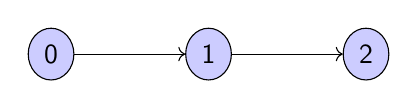
\begin{tikzpicture}
        \node[cloud] (1) {0};
        \node[cloud] (2) [right of=1,node distance=2cm] {1};
        \node[cloud] (3) [right of=2,node distance=2cm] {2};
        \draw[->] (1) -- (2);
        \draw[->] (2) -- (3);
     \end{tikzpicture}
 \end{center}
 Hence the algorithm gives wrong results if there was a cycle in the graph.
 \newpage
 \section*{Question 3}
 \subsection*{a)}
 \textbf{Disjoint Sets}: Given a set S and a collection C = \{S$_1$, S$_2$,$\dots$,S$_m$\} of subsets of S, and a number k, are there k pairwise disjoint subsets in C?\vspace*{1em}\\
 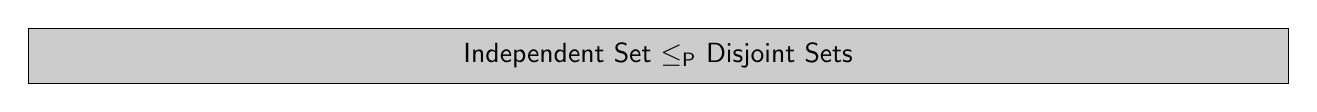
\begin{tikzpicture}
    \node[lemma] (1) {Independent Set $\leq_\text{P}$ Disjoint Sets};
 \end{tikzpicture}
 \textbf{Proof}: Suppose we have access to a black box that can solve Disjoint Sets and consider an arbitrary instance of Independent Set specified by a Graph G = (V,E) and a number k.\\
 So, Formulating an instance of Disjoint sets where the Set S = E and the collection C is given by C = \{S$_1$, S$_2$,$\dots$,S$_m$\} where 
 \begin{equation*}
     m = |V|
 \end{equation*}
 \begin{equation*}
     S_i = \{e\ |\ u_i \in V \text{ and }e = (u_i,\text{x) and } e \in E \}
 \end{equation*}
 This way of formulating the problem is at most \textbf{O(E)} since every edge will be added to two such sets.\\
 \textbf{Claim}:There are k pairwise disjoint subsets in C $\iff$ G has a independent set of size k.\vspace*{0.5em}\\
 \textbf{Forward Direction:} Note that All sets in the collection C are subsets of S since S = E and every element in S$_i$ is in E.\\
 If S$_{i_1}$,S$_{i_2}$,$\dots$,S$_{i_l}$ are $l$ $=$ k pairwise disjoint subsets of S, then Since for some p,q,
 \begin{equation*}
     S_{i_p} \cap S_{i_q} = \phi
 \end{equation*}
 Hence,no edge from i$_p$ is incident on i$_q$ for all such pairs (p,q), so the set \{i$_1$,i$_2$,$\dots$,i$_l$\} is an independent Set.\vspace*{0.2em}\\
 \textbf{Backward Direction:} Conversely, if \{i$_1$,i$_2$,$\dots$,i$_l$\} is an independent set of size $l$ $=$ k, then the sets S$_{i_p}$ and S$_{i_q}$ are disjoint since no edge from i$_p$ is incident on i$_q$ for arbitrary p,q Hence the collection \{S$_{i_1}$,S$_{i_2}$,$\dots$,S$_{i_l}$\} are pairwise disjoint sets which means the Collection C has k pairwise disjoint subsets.
 \vspace*{1em}\\
 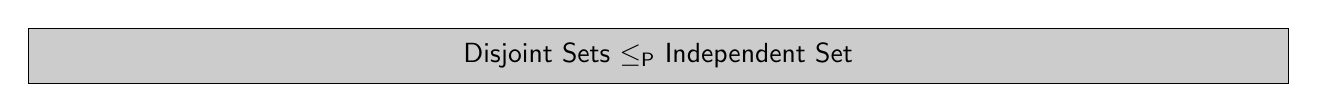
\begin{tikzpicture}
    \node[lemma] (1) {Disjoint Sets $\leq_\text{P}$ Independent Set};
 \end{tikzpicture}
 \textbf{Proof}: Suppose we have access to a black box that can solve Independent Sets and consider an arbitrary instance of Disjoint Sets specified by a Collection C = \{S$_1$, S$_2$,$\dots$,S$_m$\} of subsets of S and a number k.\\
 So Formulating as an independent set problem given by G = (V,E) where 
 \begin{equation*}
     V = \{u_i\ |\ 1 \leq i \leq m \}
 \end{equation*}
 \begin{equation*}
     E = \{(u_i,u_j)\  | \ S_i \cap S_j \neq \phi \}
 \end{equation*}
 This way of formulating the Problem is at most \textbf{O(m$^2|$S$|$)} since m$^2$ such pairs need to be checked and might be checked at most for each element in S which is polynomial.\\
 \textbf{Claim}: G has a independent set of size  k. $\iff$ There are  k pairwise disjoint subsets in C \vspace*{0.5em}\\
  \textbf{Forward Direction:} Suppose G has an independent set of Size \{i$_1$,i$_2$,$\dots$,i$_l$\}, l $=$ k then the Collection \{S$_{i_1}$,S$_{i_2}$,$\dots$,S$_{i_l}$\} is pairwise disjoint since no edge is present between i$_p$ and i$_q$ for arbitrary p,q. Hence 
 \begin{equation*}
    S_{i_p} \cap S_{i_q} = \phi, \text{ for any p,q less than }l 
 \end{equation*}
 \textbf{Backward Direction:} Conversely if \{S$_{i_1}$,S$_{i_2}$,$\dots$,S$_{i_l}$\} is a collection of $l$ $=$ k sets which are pairwise disjoint then \{i$_1$,i$_2$,$\dots$,i$_l$\} is an independent set in the graph because there is no edge between any two nodes in this set due to the construction.\\
 \subsection*{b)}
 \textbf{Dominating Sets}: Given a graph G and a number k, does G contain a dominating set of size at most k? A dominating set is a subset of vertices such that every vertex not in the subset is adjacent to some vertex in the subset.\vspace*{1em}\\
 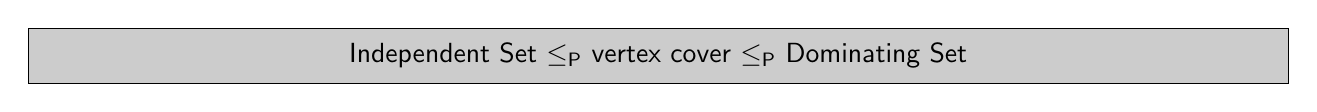
\begin{tikzpicture}
    \node[lemma] (1) {Independent Set $\leq_\text{P}$ vertex cover $\leq_\text{P}$ Dominating Set};
 \end{tikzpicture}
 \textbf{Proof}: From the Book we already know that Independent Set $\leq_\text{P}$ vertex cover. Now suppose we have access to a black box that can solve Dominating Sets and consider an arbitrary instance of vertex cover specified by a Graph G = (V,E)\vspace*{0.2em}\\
 Formulating this as an instance of Dominating Sets specified by a Graph G' = (V',E') where 
 \begin{equation*}
      V^- = \{ u\ | \ (u,v) \text{ not in } E\  \forall\  v \in V \} 
 \end{equation*}
 \begin{equation*}    
      \ V^* = \{ e_{uv} \ |\ (u,v) \in E \} \text{ and V' =} V \cup V^* - V^-
 \end{equation*}
 \begin{equation*}
     E' = \{\ (u,e_{uv}),(e_{uv},v) \ | \ (u,v) \in E \} \ \cup \ E
 \end{equation*}
 This way of formulating the problem is at most \textbf{O(E)} since we add a edge for every pair of nodes in V$^*$ and the nodes are also of \textbf{O(E+V)} and hence is polynomial reduction.\\
 \textbf{Claim}: There is a vertex cover of size k $\iff$ There is a Dominating Set of size at most k\vspace*{0.2em}\\
 \textbf{Forward Direction:} Suppose, There is a vertex cover T = \{i$_1$,i$_2$,$\dots$,i$_k$\} then we say that T' = T - V$^-$ is a dominating set of Graph G',i.e every vertex not in T' is dominated( adjacent to some vertex in T').\\
 Since Every edge is covered by a vertex cover all vertices not in T' and in V - V$^-$ are dominated by the set T' since each vertex in V - V$^-$ has an edge covered by T'.\\
 Now every vertex in V$^*$ is also dominated by T' since each edge in E is covered by T' alone since the vertices with 0 edges do not contribute, Hence there is at least one vertex v from V - V$^-$ in T' for every edge e in E. This vertex dominates the new vertex introduced for every edge in V$^*$.\\
 Hence, T' = T - V$^-$ is a dominating set of Graph G' since it dominates all vertices present in the Graph.\vspace*{0.2em}\\
 \textbf{Backward Direction:} Conversely, If T = \{i$_1$,i$_2$,$\dots$,i$_l$\} is a dominating set of Graph G' of size l = k - $|$V$^-|$ then T' = T + V$^-$ is a vertex cover of size k of the Graph G.\\
 It is safe to assume no vertex from V$^*$ is in T since if there was a vertex x in T it can always be replaced by one of its neighbours since x can dominate only u and v if (u,x) and (x,v) lie in E'. Now if we replace x with u and v is not dominated by any other vertex, u dominates x and v since there is an edge (u,v) in the graph.\\
 So, all vertices from T are from  V - V$^-$ and since all vertices are dominated by the set T.\\
 For every edge (u,v) in G, since e$_{uv}$ is dominated by T either u or v must be there in T which implies T is a vertex cover of G.\\
 {\large Hence, vertex cover of size k can be determined if there exists a dominating cover of size at most k.}
 \vspace*{1em}\\
 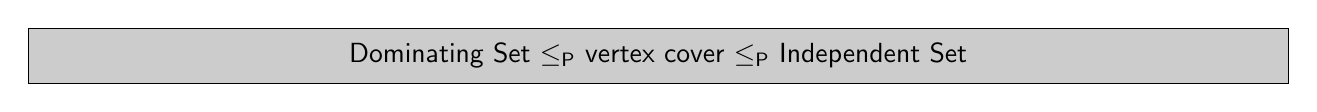
\begin{tikzpicture}
    \node[lemma] (1) {Dominating Set $\leq_\text{P}$ vertex cover $\leq_\text{P}$ Independent Set};
 \end{tikzpicture}
 \textbf{Courtesy:} \href{https://cstheory.stackexchange.com/questions/25376/is-there-simple-reduction-dominating-set-to-vertex-cover}{This} url Helped us in getting the idea below. Thanks!!\\
 \textbf{Proof}: From the book we already know that vertex cover $\leq_\text{P}$ Independent Set. Now suppose we have access to a black box that can solve Vertex Cover and consider an arbitrary instance of Dominating Sets Sets specified by a Graph G = (V,E) and a number k.
 \newpage
 Assuming that there are no zero degree vertices\\
 Formulating this as an instance of Vertex Cover specified by a Graph G' = (V',E') where 
 \begin{equation*}
     V_1 = \{u_{ij}\ |\ 1\leq i,j\leq n \} 
 \end{equation*}
 \begin{equation*}
     V_2 = \{u_{ij}' \ | \ (i,j) \not\in E \}
 \end{equation*}
 \begin{equation*}
     V' = V \cup V_1 \cup V_2
 \end{equation*}
 \begin{equation*}
     E_1 = \{(u_{ij},u_{ik}) \ | \ \forall i, j\neq k \}
 \end{equation*}
 \begin{equation*}
     E_2 = \{(u_i,u_{ii})\ | \ \forall i \}
 \end{equation*}
 \begin{equation*}
     E_3 = \{(u_i,u_{ji})\ | \ \forall (i,j) \in E \}
 \end{equation*}
 \begin{equation*}
     E_4 = \{(u_{ij},u_{ij}')\ | \ \forall (i,j) \not\in E \}
 \end{equation*}
 \begin{equation*}
     E' = E_1 \cup E_2 \cup E_3 \cup E_4
 \end{equation*}
 Note that this reduction is Polynomial because each of the sets mentioned above can be made in polynomial time which takes at most \textbf{O(n$^2$+E)} and hence is a polynomial reduction\\
 \textbf{Claim}: There exists a vertex cover in G' of size n$^2$ - n + k $\iff$ There is a dominating set in G of size at most k.\vspace*{0.5em}\\
 \textbf{Forward Direction:} Suppose that there is vertex cover T of size n$^2$ - n + k, remove all the vertices of the from $u_{ij}$ where (i,j) is not in E, these cannot be more than k in number which is due to the clique property below.\\
 Firstly Note that there are n cliques in the graph, This is due to the Edge set $E_1$. Hence for a vertex cover to cover all edges of $E_1$ there must be at least n-1 vertices from each clique leading to n(n-1) vertices in all to cover edges from Edge Set $E_2$.\\
 If Some clique has all n vertices then we can safely replace one of its vertex by its neighbours from set V which doesn't affect the vertex covering property of the Set.\\
 Now remove all vertices from these cliques,i.e n(n-1) in number,Now we remain with a set T' of size $\leq$ k\\
 This Set T' has vertices only from V and we say that this set is dominating set in The graph G\\
 Since T was a vertex cover, all edges from G' must be covered by T, we can say that T' is a dominating set since edges from $E_3$ must be covered by the Set T which means due to the construction for every $(u_i,u_{ji})$ there is an edge (i,j) in G' which means $u_i$ and $u_j$ are adjacent.
 Hence there exists at least one vertex in set T' such that every vertex not in T' is adjacent to it by the above claim
 \vspace*{0.25em}\\
 \textbf{Backward Direction:} Suppose there is a dominating set T of size l (at most k) in Graph G then select all vertices from the clique except the one that is adjacent to a selected $u_i$ in the Set T to get T' and for $u_i$ not in the set T we add all vertices from the ith clique except the one adjacent to the vertex $u_i$ (we can be sure of its existence since the Set T is a dominating set) and add any arbitrary k-l vertices from the set $V_2$ to make the size of the new Set T'' equal to n$^2$ - n + k.\\
 T' will be a vertex cover since every vertex not in T from V is dominated by the set T and hence from all $u_i$ from the set T there will be edges to all $u_{ji}$ which makes the edge Set $E_3$ also get covered by the set T'. $E_4 $ is already covered since we are not leaving out any vertex of the form $u_{ij}$ where (i,j) is not in E due to the construction of T'.\\
 $E_2$ is covered since for every $u_i$ either $u_i$ or $u_{ii}$ belongs to the set T'.\\
 $E_3$ is also covered since from all n cliques in the Graph G, n-1 vertices from each clique cover all edges except those of the form $u_i$ to $u_{pi}$ where $u_{pi}$ was left out but since T was a dominating set the edges $u_i$ to $u_{pi}$ will be covered and hence T' will be a vertex cover in Graph G'.\\
 T'' will be a vertex cover since adding vertices from $V_2$ to T' doesn't make any change since T' is already a vertex cover.\vspace*{0.8em}\\
 {\large Hence, dominating set of size at most k can be determined if there exists a vertex cover of size n$^2$-n+k.}
 \subsection*{c)}
 \textbf{Problem C} :Given a graph G, and a number k, is there a subset of k vertices in G such that there is no path of length at most 2 between any two vertices in the subset.\vspace*{1em}\\
 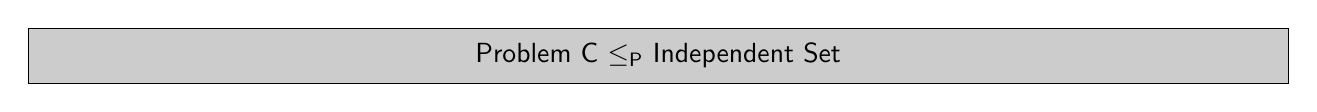
\begin{tikzpicture}
    \node[lemma] (1) {Problem C $\leq_\text{P}$ Independent Set};
 \end{tikzpicture}
 \textbf{Proof}: Suppose we have access to a black box that can solve Independent Sets and consider an arbitrary instance of Problem C specified by a Graph G = (V,E) and a number k.\\
 Formulating this problem as an Independent Set Problem specified by the Graph G' = (V,E') where 
 \begin{equation*}
     E' = E \cup \{\text{ (u,v) } | \text{ (u,w) and (w,v) }\in E \ \}
 \end{equation*}
 This way of formulating the Problem can be done in at most \textbf{O(E$^2$)} by checking for every pair of edges possible for a common vertex and hence is polynomial reduction.\\
 \textbf{Claim}: G has a subset of size k such that there is no path of length at most 2 between any two vertices in the subset $\iff$ G' has a independent Set of Size k.\vspace*{0.5em}\\
\textbf{Forward Direction:} Suppose G' has an independent set of Size T = \{i$_1$,i$_2$,$\dots$,i$_k$\}, then we can say that there is no such edge (i$_p$,i$_q$) because the set is independent.\\
 Now suppose there exists a node v $\in$ V, such that (i$_p$,v) and (v,i$_q$) belong to the Edge Set E.\\
 Then by construction of E', (i$_p$,i$_q$) $\in$ E' Which means the set becomes not independent\\ Hence,There exists no such bridge node v.\\
 Hence, if there exists a path P from (i$_p$,i$_q$) then $|$P$|$ $\geq$ 3.\\
 Therefore the Set T serves the required Purpose.\vspace*{0.2em}\\
 \textbf{Backward Direction:} Suppose G has a Set T = \{i$_1$,i$_2$,$\dots$,i$_k$\}, then we can say that there is no edge (i$_p$,i$_q$) in E and there is no node v such that (i$_p$,v) and (v,i$_q$) belong to the Edge Set E since Path length $>$ 2.\\
 Hence by construction, We can say that there is no such edge (i$_p$,i$_q$) in E'. Hence the set T itself satisfies to be a Independent Set in the new Graph G'.
 \vspace*{1em}\\
 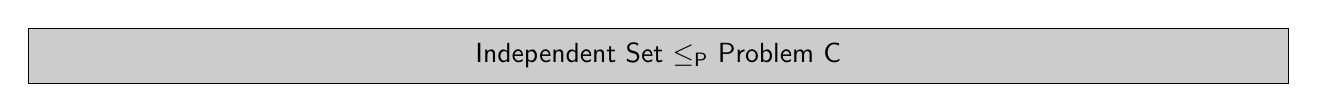
\begin{tikzpicture}
    \node[lemma] (1) {Independent Set $\leq_\text{P}$ Problem C};
 \end{tikzpicture}
 \textbf{Proof}: Suppose we have access to a black box that can solve Problem C and consider an arbitrary instance of Independent Sets Specified by a Graph G = (V,E) and a number k.\\
 Formulating this problem as an instance of Problem C specified by the Graph G' = (V',E') where
 \begin{equation*}
     V^* = \{ e_{uv} \ |\ (u,v) \in E \} \text{ and V' =} V \cup V^*
 \end{equation*}
 \begin{equation*}
     E' = \{\ (u,e_{uv}),(e_{uv},v) \ | \ (u,v) \in E \} \ \cup \{\ (x,y)\ | \ x,y \in V^* \}
 \end{equation*}
 This way of formulating the problem is at most \textbf{O(E$^2$)} since we add a edge for every pair of nodes in V$^*$ and the nodes are also of \textbf{O(E+V)} and hence is polynomial reduction.\\
 \textbf{Claim}: G has a independent Set of Size k  $\iff$  G' has a subset of size k such that there is no path of length at most 2 between any two vertices in the subset \vspace*{0.5em}\\
 \textbf{Forward Direction:} Suppose G has an independent Set T = \{i$_1$,i$_2$,$\dots$,i$_k$\} ,then there is no such edge (i$_p$,i$_q$). Hence there is no such path of length less than 3 in the new graph between the vertices since there must be at least three nodes in between since there is no node x such that (i$_p$,x),(x,i$_q$) $\in$ E'.\vspace*{0.2em}\\
 \textbf{Backward Direction:} Suppose G' has a Set T = \{i$_1$,i$_2$,$\dots$,i$_k$\} satisfying Problem C. Note that no two vertices from V$^*$ do not belong to this set since they have a direct edge between them.\\
 Now If there was some vertex v from V$^*$, then it can always replaced by one of its neighbours, say t, This is because any neighbour of t,$\mu$ in G do not belong to the set T because they have a path of length 2 from vertex v i.e vg$_{t\mu}\mu$.Hence no there is no path of length $<$ 2 from t \\
 Hence it is safe to assume all vertices in the set T are from V.\\
 Then we can say that there is no edge (i$_p$,i$_q$) in E' and there is no node x such that (i$_p$,x) and (x,i$_q$) belong to the Edge Set E' since Path length $>$ 2.\\
 Therefore We have no such edge (i$_p$,i$_q$) due to the construction since these are from V and not V$^*$.\\
 Hence the set T = \{i$_1$,i$_2$,$\dots$,i$_k$\} is an independent Set in the Graph G.
 \subsection*{d)}
 \textbf{Edge Disjoint Subtrees}: Given a tree T, and a collection \{T$_1$, T$_2$,$\dots$, T$_m$\} of subtrees of T, are there k edge-disjoint subtrees in the given collection?\vspace*{0.5em}\\
 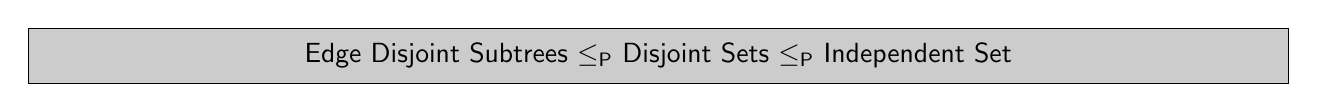
\begin{tikzpicture}
    \node[lemma] (1) {Edge Disjoint Subtrees $\leq_\text{P}$ Disjoint Sets $\leq_\text{P}$ Independent Set};
 \end{tikzpicture}
 \textbf{Proof}:  Suppose we have access to a black box that can solve Disjoint Sets and consider an arbitrary instance of Edge DisJoint Subtrees specified by a Tree T and a collection C = \{T$_1$, T$_2$,$\dots$, T$_m$ \} of subtrees of T and a number k.\vspace*{0.2em}\\
 Formulating this as an Disjoint Set Problem specified by a Set S and a collection C' =\{S$_1$, S$_2$,$\dots$,S$_m$\} where
 \begin{equation*}
     S = \{ e \ | \ e \text{ is an edge in T} \}
 \end{equation*}
 \begin{equation*}
     S_i = \{ e \ |\  e \text{ is an edge in T}_i\}
 \end{equation*}
 This reduction is polynomial in Time as it takes at most \textbf{O(mV)} time to frame the sets from T if T is not in adjacency list representation.\vspace*{0.2em}\\
 \textbf{Claim}: k edge-disjoint subtrees $\iff$ k pairwise disjoint subsets \vspace*{0.2em}\\
 This is obvious since an edge is present in two sets if and only if it is present in both the corresponding Trees and hence as a result of this the Two statements are equivalent.\\
 Hence Edge Disjoint Subtrees $\leq_\text{P}$ Disjoint Sets,Since in part a we have already proven that  Disjoint Sets $\leq_\text{P}$ Independent Set we can say edge Disjoint subtrees $\leq_\text{P}$ Independent Set.
 \vspace*{1em}\\
 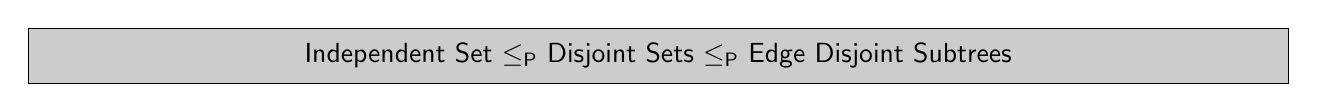
\begin{tikzpicture}
    \node[lemma] (1) {Independent Set $\leq_\text{P}$ Disjoint Sets $\leq_\text{P}$ Edge Disjoint Subtrees};
 \end{tikzpicture}
 \textbf{Proof}: Suppose we have access to a black box that can solve Edge Disjoint Subtrees and we have an reduced instance of Disjoint Sets from Independent Set Problem specified by a set S and a collection of subsets of S, C = \{S$_1$, S$_2$,$\dots$,S$_m$\} and a number k.\vspace*{0.2em}\\
 Formulating this as an instance of Edge Disjoint Subtree problem specified by T = (V,E) and a collection C' = \{T$_1$, T$_2$,$\dots$, T$_m$ \} where 
 \begin{equation*}
     V = \{s\} \cup \{ u_i \ | \ i \in S \}
 \end{equation*}
 \begin{equation*}
     E = \{ (s,u_i) \ | \ i \in S \}
 \end{equation*}
 \begin{equation*}
     T_i = (V_i,E_i) \text{ where } V_i = \{s\} \cup \{ u_j \ | \ j \in S_i \} \text{ and } E = \{ (s,u_j) \ | \ j \in S_i \}
 \end{equation*}
 This way of formulating the problem is at most \textbf{O(mS)} which is polynomial and hence a polynomial reduction.\vspace*{0.2em}\\
 \textbf{Claim}: k  pairwise disjoint Subsets $\iff$ k edge-disjoint subtrees\vspace*{0.5em}\\
 Firstly note that T is a Tree with $|$S$|$ edges and the number of vertices in the Graph is  $|$S$|$ + 1 and it is connected and hence a Tree.\\
 Similarly T$_i$ is also a tree since number of edges = number of vertices - 1 and the Graph so formed is a Tree. T$_i$ is a subtree of T since V$_i$ $\subset$ V and E$_i$ $\subset$ E. Hence T$_i$ is a subtree of T.\\
 Suppose two subsets in Collection C S$_p$ and S$_q$ are pairwise disjoint, then we have no edge common for Trees T$_p$ and T$_q$ since no vertex of the Tree is common to both S$_p$ and S$_q$.\\
 Hence if there are k pairwise disjoint subsets in C, then there are k edge disjoint subtrees in collection C'.\vspace*{0.5em}\\
 Suppose two trees T$_p$ and T$_q$ in collection C' have no common edge which means there is no common element of S$_p$ and S$_q$ since edges are of the format (s,x) for any x Hence S$_p$ and S$_q$ are pairwise disjoint subsets.\\
 Hence if there are k edge disjoint subtrees in C', then there are k pairwise disjoint subsets in collection C.\vspace*{0.5em}\\
 \subsubsection*{Vertex Disjoint Subtrees}
 Let the vertices in T be \{$u_i$ $|$ 1 $\leq$ i $\leq$ n\}.\\
 Without loss of generality we can assume the tree to be rooted at $u_r$, where there is no incoming edge to $u_r$.\\
 Let $d_i$ denote the depth of $u_i$ in the Tree T.\\
 These can be calculated easily by using DFS from $u_r$.\\
 Let $c_i$ denote the list of all nodes which have directed edges of the from ($u_i$,x), which are known as children of the Tree. This can also be calculated easily by a DFS from $u_r$.\\
 Let $r_j$ denote the root of the Subtree T$_j$ which can be calculated by finding the vertex with the least $d_i$. This is unique since T$_j$ is a subtree.\\
 Let $L_j$ denote the list of leaves of the Subtree T$_j$ which can be easily calculated using DFS on T$_j$ after finding the root of this Tree $r_j$. A leaf is a node which has no outgoing edge.\\
 Let $\lambda_i$ be the maximum vertex disjoint subtrees from the collection C = \{T$_1$, T$_2$,$\dots$, T$_m$ \} in subtree rooted at $u_i$.\\
 Let $V(T_j)$ denote the vertex set of $T_j$ and Let $\sum_{x}^{X} g(x)$ denote the sum of g(x) over the set X
 \begin{equation*}
     \lambda_i = \max(\sum_{j \in c_i} \lambda_j,\Lambda_{ij})
 \end{equation*}
 \begin{equation*}
     \Lambda_{ij} = \max_{u_i\text{ is root of }T_j }(1 + \sum_k^{L_j}\sum_l^{c_k} \lambda_l + \sum_{m \in c_i}^{V(T_j)} \lambda_m)
 \end{equation*}
 By this recursive relation, we can calculate $\lambda_r$ i.e for the root of the original tree.\\
 If $\lambda_r$ $\geq$ k, then we have k vertex disjoint Subtrees else we cannot have k set of vertex disjoint Subtrees.\\
 \vspace*{0.5em}\\
 \textbf{Correctness}: \\
 In the calculation of $\lambda_i$,\\
 If $u_i$ is not there in the maximum number of vertex disjoint Subtrees, then maximum number of disjoint subtrees will be $\sum_{j \in c_i} \lambda_j$.\\
 This is due to the reason that every subtree in the subtree collection C should be in any one of the branches.\\
 If $u_i$ belongs to any one of those subtrees say T$_j$, then remaining subtrees must be in the branches in which $T_j$ doesn't contain a vertex(from $L_j$ or they should be from the Trees rooted at the leaves of $T_j$ which ensures that $u_i$ doesn't belong to other subtrees.\\
 This quantity is exactly computed by $\Lambda_{ij}$ for a given vertex $u_i$ and the subtree T$_j$ whose root is $u_i$\\
 \begin{equation*}
     \Lambda_{ij} = \max_{u_i\text{ is root of }T_j }(1 + \sum_k^{L_j}\sum_l^{c_k} \lambda_l + \sum_{m \in c_i}^{V(T_j)} \lambda_m)
 \end{equation*}
 \textbf{Time Analysis}:\\
 
 For Calculating $d_i$ and $c_i$ it takes O(n) as we do DFS for the Tree T rooted at $u_r$, i.e DFS($u_r$)\\
 The root of a Tree can be calculated in O(n) as comparing depth of each would give us the answer\\
 Hence for m Trees from the Collection the roots can be calculated in O(mn) Time.\\
 We follow a Dynamic Programming based approach by following the order in a DFS ,i.e we first calculate for each leave and then move one level up and then calculate for this level and so on.\\
 To Calculate $\lambda_i$ from the recursion relation, we need the max of Two quantities one which can be computed in O(n) time and the other $\Lambda_{ij}$ which can be computed in O(mn) time.\\
 Hence Time complexity for $\lambda_i$ is O(n+mn).\\
 For Calculating all $\lambda_i$ it takes O(n$^2$+mn$^2$).\\
 Hence the Time complexity of this approach is \textbf{O(n$^2$+mn$^2$)} and Hence a Polynomial Time Algorithm.\\
 \end{document}
